\subsection{UNet}
\label{sec:aj_unet}

U-Net is a fully convolutional encoder-decoder architecture originally designed for biomedical image segmentation\,\cite{b13}. Its symmetric design with skip connections enables precise boundary localisation by combining high-level semantic features with low-level spatial details. Our implementation extends the classical U-Net to leverage multi-spectral imagery and domain-specific spectral indices.\footnote{this is why we choose not to bruteforce a fantastic perfomance with \hyperlink{https://github.com/MIC-DKFZ/nnUNet}{nnUNet}; \emph{domain-knowledge}.}

\begin{figure}
  \centering
  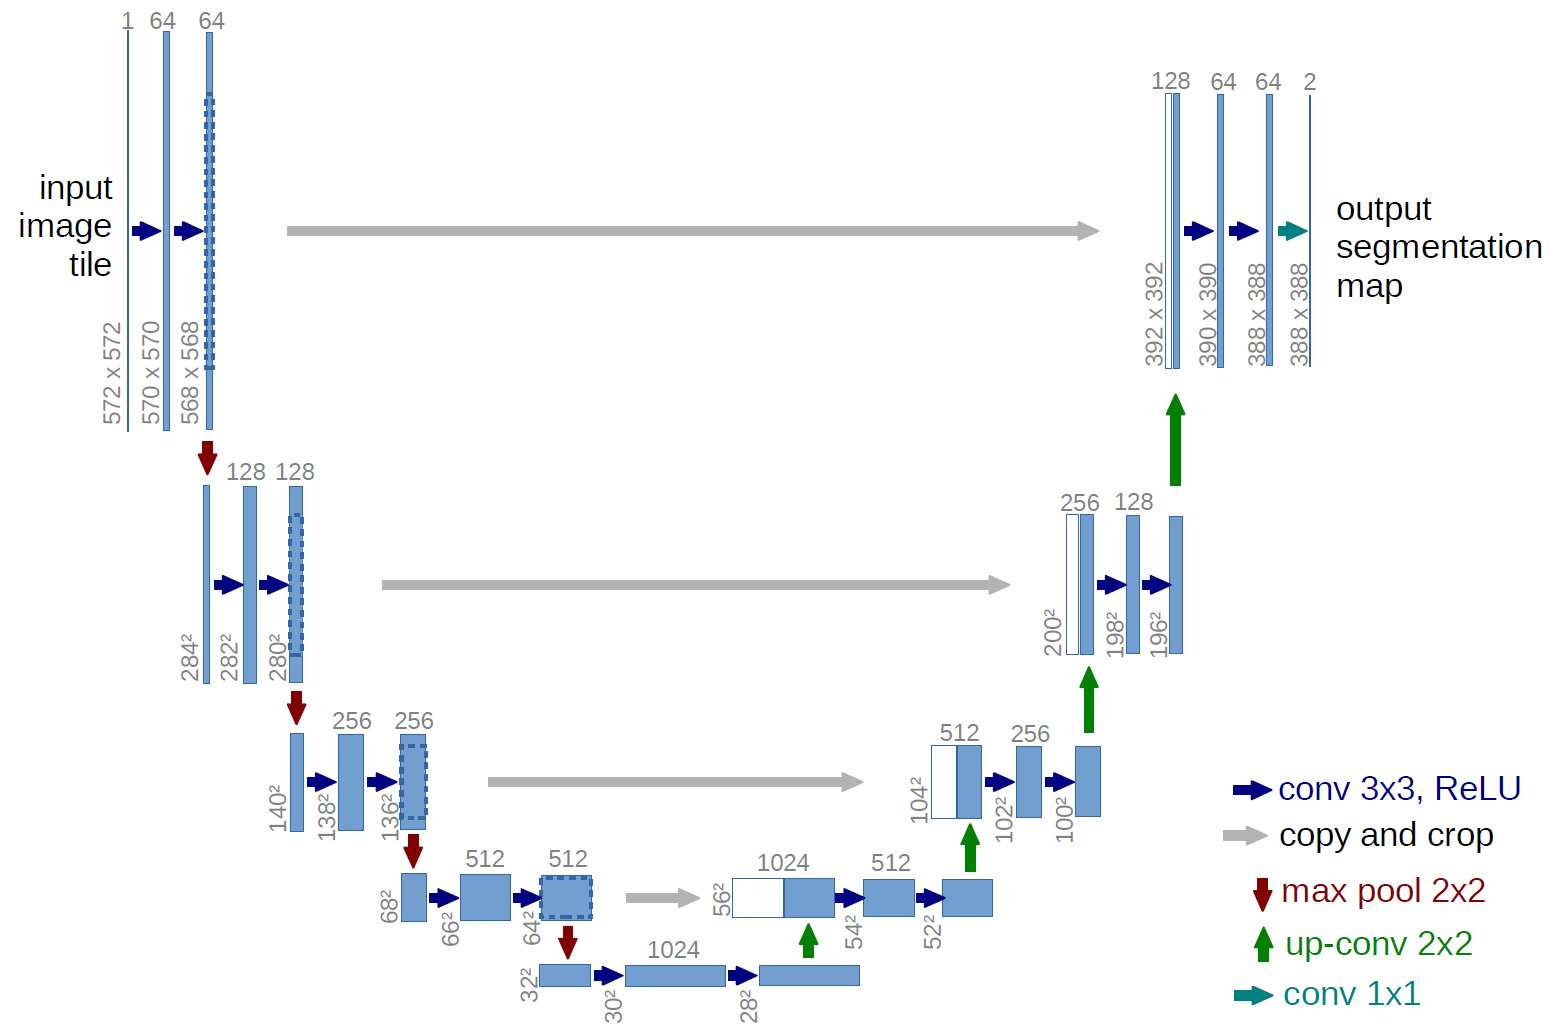
\includegraphics[width=.9\linewidth]{figs/unet-proto.jpg}
  \caption{Prototypical UNet Architecture}
  \label{fig:unet_proto}
\end{figure}

\paragraph{Motivation.}
Dead trees exhibit distinct spectral signatures across visible and near-infrared bands. Healthy vegetation reflects strongly in NIR while absorbing in red wavelengths, whereas stressed or dead vegetation shows reduced NIR reflectance. By incorporating both RGB and NRG (Near-infrared, Red, Green) channels alongside computed spectral indices, we provide the network with domain-specific features that enhance dead tree discrimination.

\paragraph{Multi-Channel Input Pipeline.}
Our dataset loader constructs 8-channel inputs by concatenating RGB channels, NRG channels, and two computed spectral indices:

\begin{lstlisting}[language=Python]
# extract individual channels for spectral indices
# RGB: R=0, G=1, B=2
# NRG: N=0, R=1, G=2 (NIR, Red, Green in NRG image)
red = rgb_tensor[0:1]      # red rgb
green = rgb_tensor[1:2]    # green rgb  
blue = rgb_tensor[2:3]     # blue rgb
nir = nrg_tensor[0:1]      # nir, nrg

# NDVI: (nir - red) / (nir + red)
eps = 1e-8 # div by 0 error
ndvi = (nir - red) / (nir + red + eps)

# ndwi = (green - nir) / (green + nir)  
ndwi = (green - nir) / (green + nir + eps)

# concatenating:
image_8ch = torch.cat([rgb_tensor, nrg_tensor, ndvi, ndwi], dim=0)  # (8, H, W)
\end{lstlisting}

The Normalised Difference Vegetation Index (NDVI)\,\cite{b14} and Normalised Difference Water Index (NDWI)\,\cite{b15} are computed as:
\begin{align}
  \text{NDVI} &= \frac{\text{NIR} - \text{Red}}{\text{NIR} + \text{Red}}, \\
  \text{NDWI} &= \frac{\text{Green} - \text{NIR}}{\text{Green} + \text{NIR}}.
\end{align}

NDVI quantifies vegetation health and photosynthetic activity, with values near +1 indicating healthy vegetation and values near -1 or 0 indicating stressed or dead vegetation. NDWI captures water stress in vegetation, providing complementary information for dead tree identification.

\begin{figure}
  \centering
  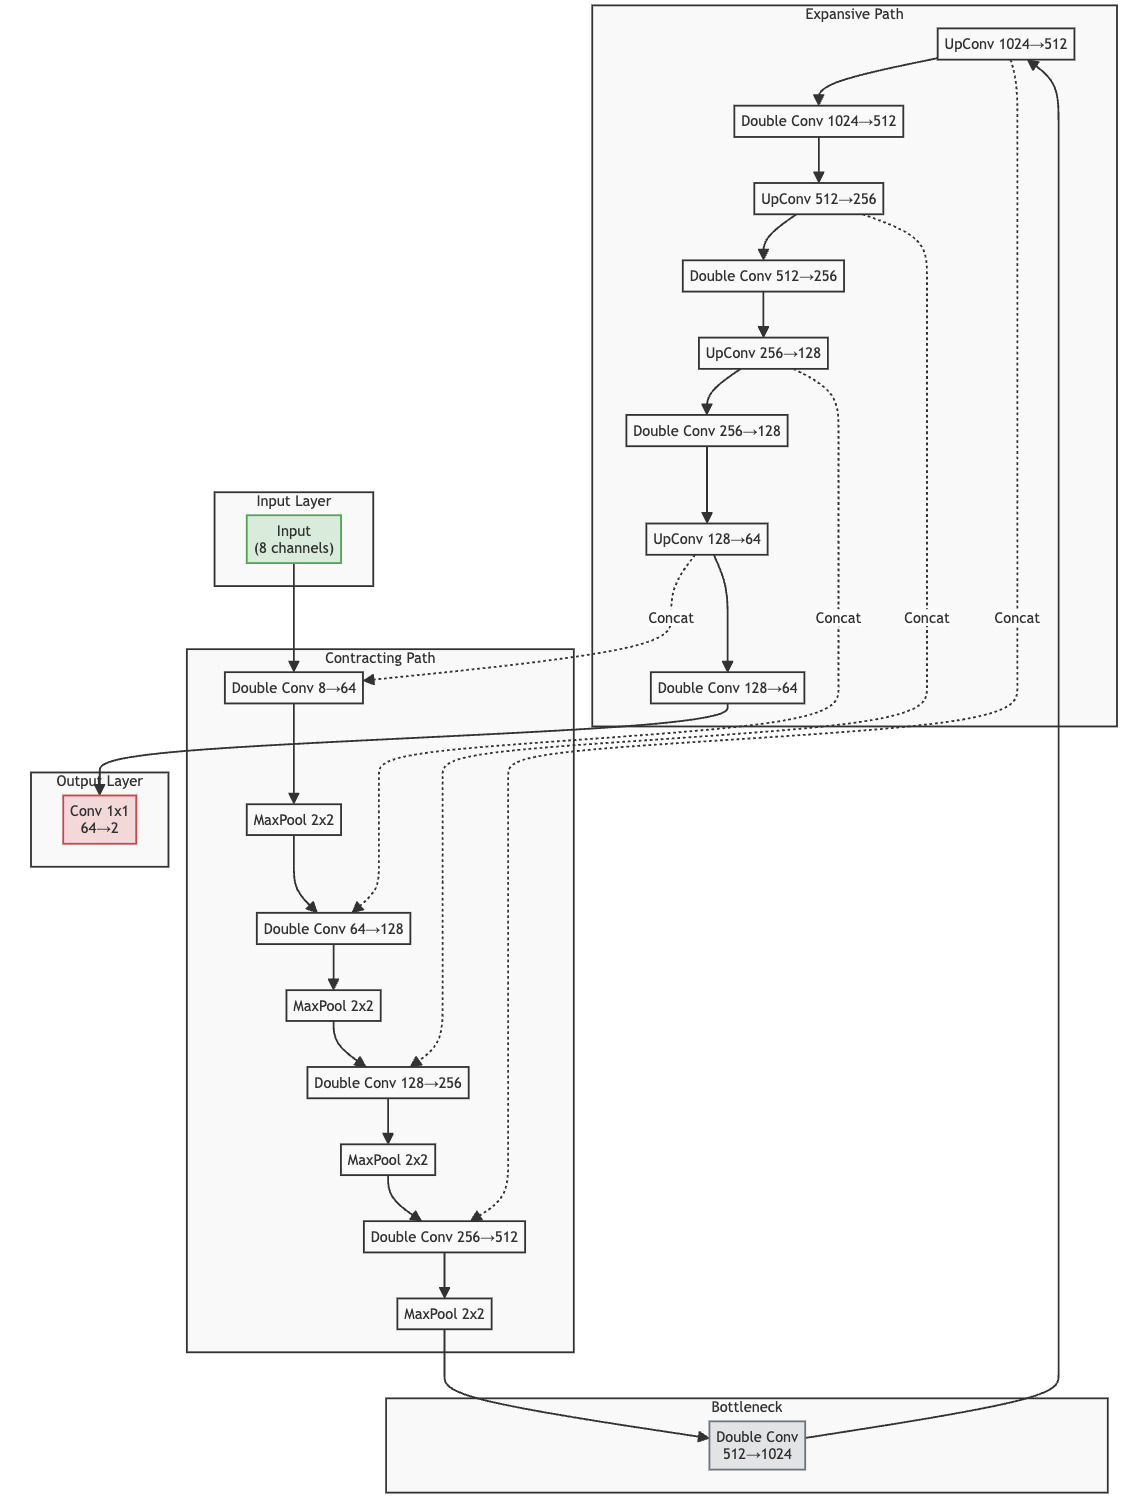
\includegraphics[width=.9\linewidth]{figs/unet-merm.jpg}
  \caption{UNet architecture: 8-channel encoder-decoder with skip connections. The contracting path captures context while the expansive path enables precise localisation. Visualisation, courtesy of torchviz \cite{b16} and Claude \cite{b17}}
  \label{fig:aj_unet_arch}
\end{figure}

\paragraph{Network Architecture.}
The U-Net encoder consists of four downsampling stages, each containing double convolutions followed by max pooling:

\begin{lstlisting}[language=Python]
class DoubleConvolution(nn.Module):
    def __init__(self, in_channels: int, out_channels: int):
        super().__init__()
        self.first = nn.Conv2d(in_channels, out_channels, kernel_size=3, padding=1)
        self.act1 = nn.ReLU()
        self.second = nn.Conv2d(out_channels, out_channels, kernel_size=3, padding=1)
        self.act2=nn.ReLU()

    def forward(self, x: torch.Tensor):
        x = self.first(x)
        x = self.act1(x)
        x = self.second(x)
        return self.act2(x)
\end{lstlisting}

The contracting path progressively reduces spatial resolution \((256^2 \rightarrow 128^2 \rightarrow 64^2 \rightarrow 32^2 \rightarrow 16^2)\) while increasing feature channels \((8 \rightarrow 64 \rightarrow 128 \rightarrow 256 \rightarrow 512 \rightarrow 1024)\). The expansive path reverses this process via transposed convolutions, concatenating corresponding encoder features through skip connections to preserve spatial information.

\paragraph{Loss Function Design.}
Class imbalance poses a significant challenge with dead trees comprising only $\approx$3\% of pixels. We address this with a composite loss combining Dice and Focal losses:

\begin{lstlisting}[language=Python]
class CombinedLoss(nn.Module):
    def __init__(self, dice_weight=0.5, focal_weight=0.5, alpha=0.25, gamma=2.0):
        super().__init__()
        self.dice_weight = dice_weight
        self.focal_weight = focal_weight
        self.dice_loss = DiceLoss()
        self.focal_loss = FocalLoss(alpha=alpha, gamma=gamma)
        
    def forward(self, outputs, targets):
        dice = self.dice_loss(outputs, targets)
        focal = self.focal_loss(outputs, targets)
        return self.dice_weight * dice + self.focal_weight * focal
\end{lstlisting}

The combined loss is:
\begin{equation}
  \mathcal{L} = \lambda_{\text{Dice}}\mathcal{L}_{\text{Dice}} + \lambda_{\text{Focal}}\mathcal{L}_{\text{Focal}},
  \quad (\lambda_{\text{Dice}}, \lambda_{\text{Focal}}) = (0.5, 0.5),
\end{equation}

where the Focal loss term addresses class imbalance:
\begin{equation}
\mathcal{L}_{\text{Focal}} = -\alpha(1-p_t)^\gamma \log(p_t),
\end{equation}
with $\alpha = 0.25$ and $\gamma = 2.0$ to down-weight easy examples and focus learning on hard cases.

\begin{figure}
  \centering
  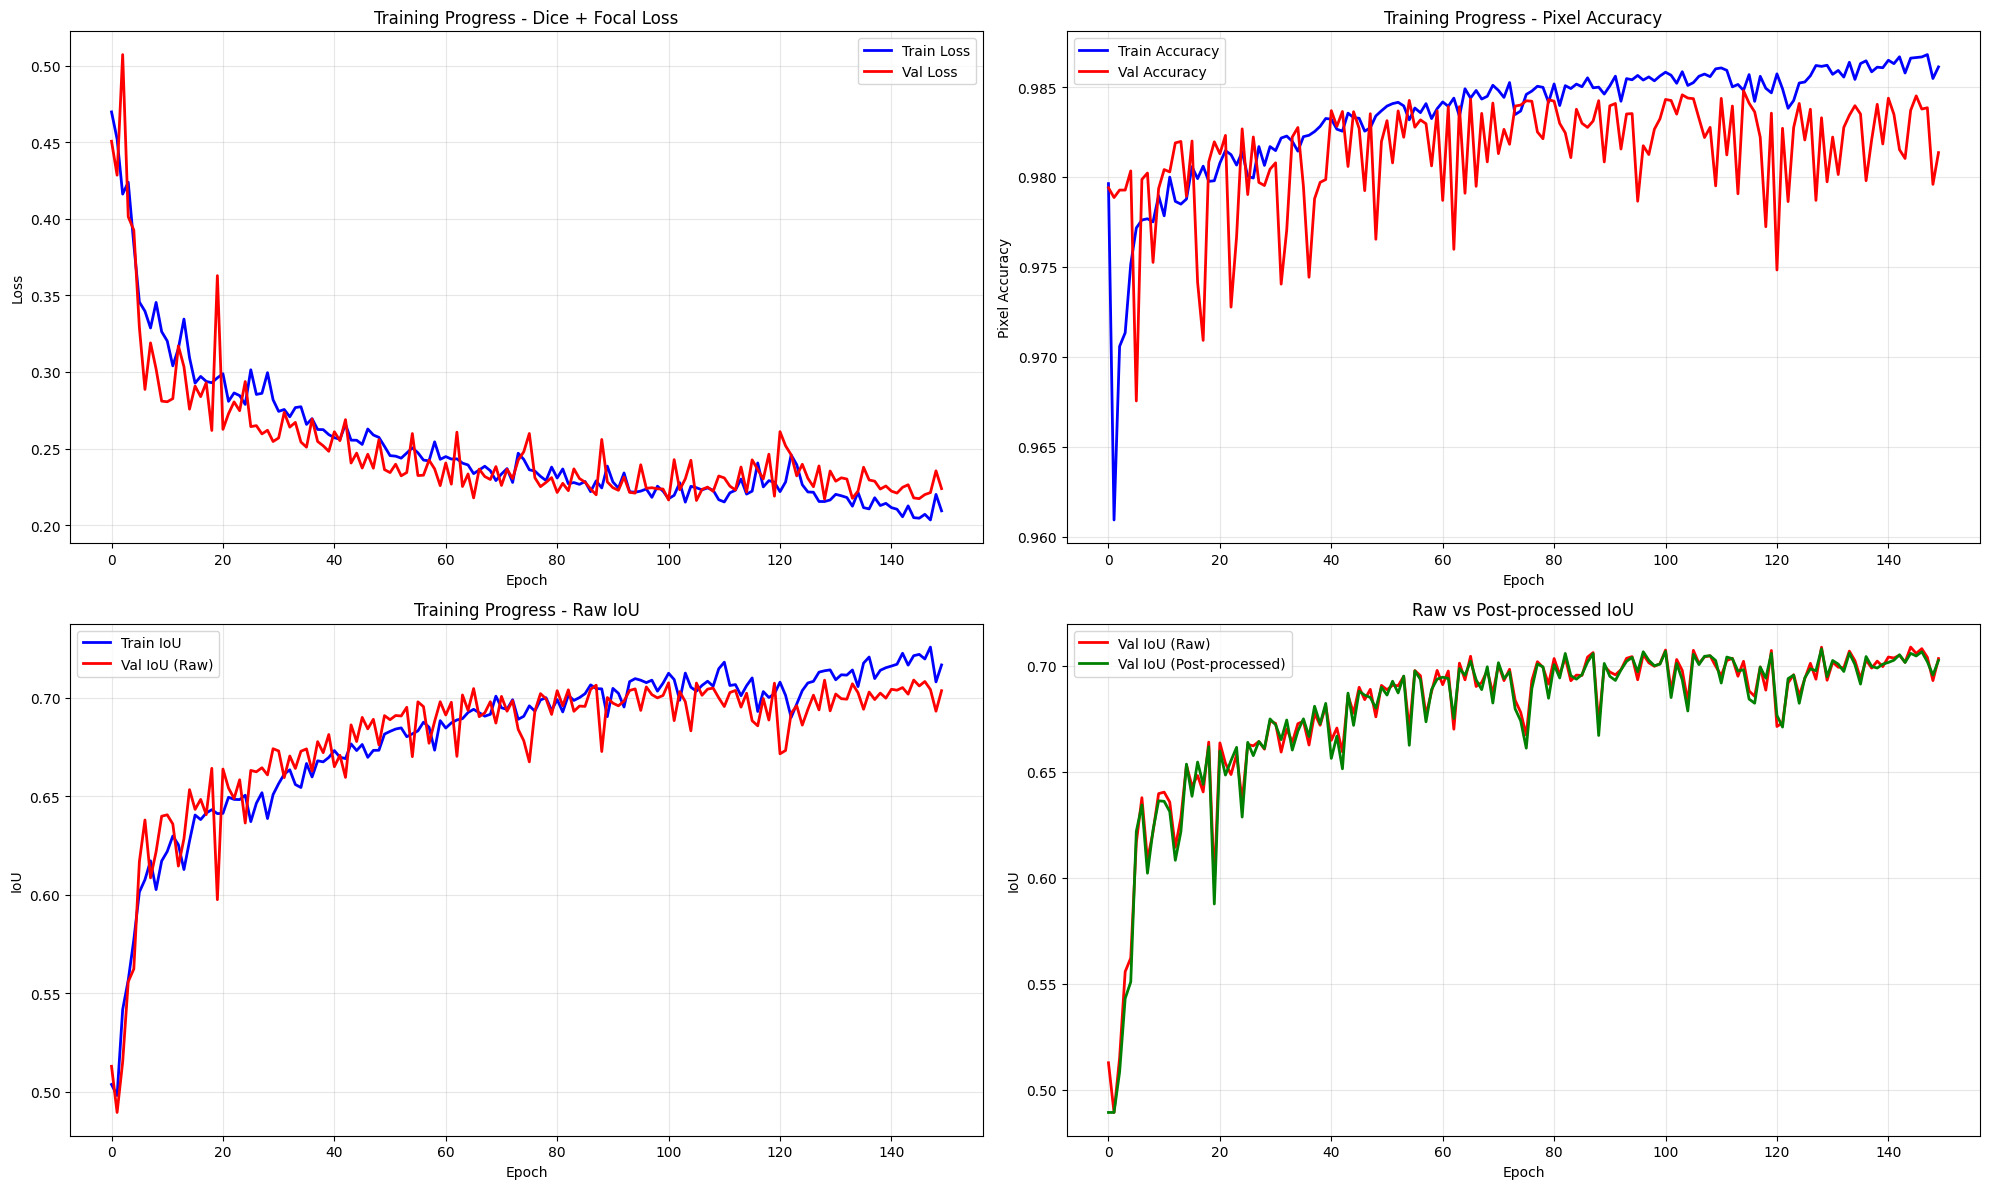
\includegraphics[width=.9\linewidth]{figs/unet-train-curve.jpg}
  \caption{Training progression showing convergence of combined Dice-Focal loss and IoU metrics over 150 epochs. Post-processing consistently improves validation IoU.}
  \label{fig:training_curves}
\end{figure}

\paragraph{Post-Processing Pipeline.}
Raw network predictions are refined through a two-stage post-processing pipeline:

\begin{enumerate}
\item \textbf{Probability Thresholding:} Dead tree probabilities are thresholded at 0.6 rather than the default 0.5, reducing false positives in ambiguous regions.
\item \textbf{Morphological Operations:} Sequential opening (erosion→dilation) removes noise, followed by closing (dilation→erosion) to fill holes in detected regions.
\end{enumerate}

This pipeline yields substantial IoU improvements ($+0.04$ typical) by cleaning spurious activations while preserving true positive detections.

\begin{figure}
  \centering
  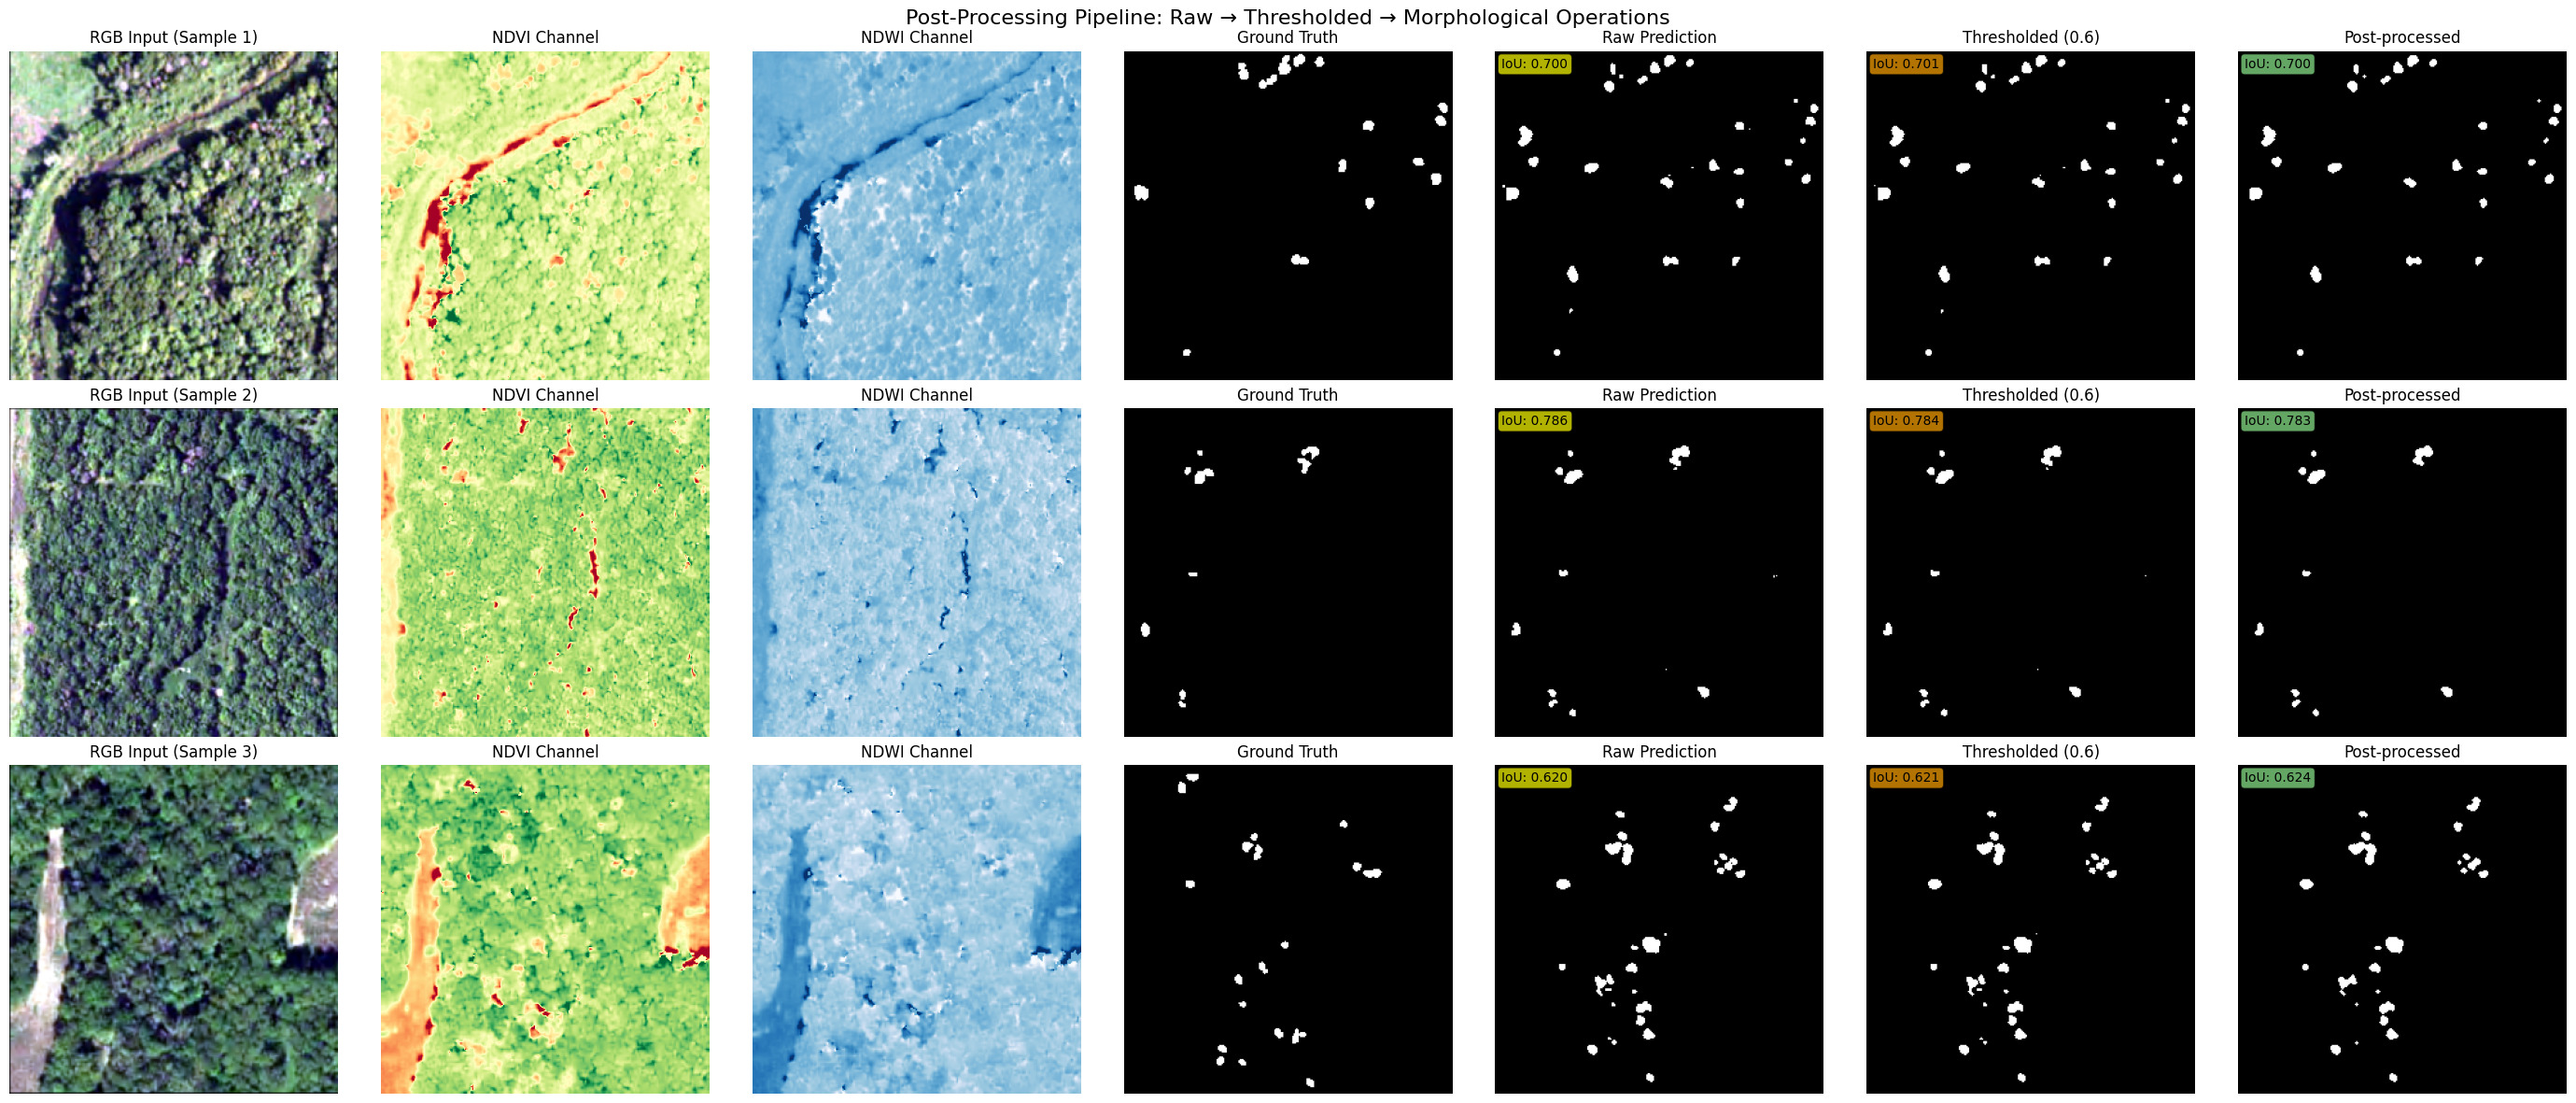
\includegraphics[width=.9\linewidth]{figs/unet-pipeline-compared.jpg}
  \caption{imperfect ablation studies:\\ raw predictions → probability thresholding → morphological cleaning}
  \label{fig:postprocessing}
\end{figure}

\paragraph{Training Configuration.}
The model was trained for 150 epochs using Adam optimiser (lr $= 10^{-3}$) with data augmentation including horizontal/vertical flips and 10° rotations. Input images were resized to $256 \times 256$ with batch size 8. All experiments were conducted on UNSW's Katana high-performance computing cluster\,\cite{b18}. The best model achieved a validation IoU of \textbf{0.7078} after post-processing, representing a significant improvement over the raw prediction IoU of 0.6634.
